\documentclass{article}
\usepackage{geometry}
\geometry{left=2cm,right=2cm,top=1cm,bottom=2cm}
\usepackage{mathtools}
\usepackage{amssymb}
\usepackage{bm}
\usepackage{verbatim}
\usepackage{float}
\renewcommand{\arraystretch}{1.3}

\title{HOMEWORK1}
\author{Runlin Hou}
\date{\today}

\begin{document}
    \maketitle
    \subsection*{Problem 1}

    (1) ER diagram
    \begin{center}
        %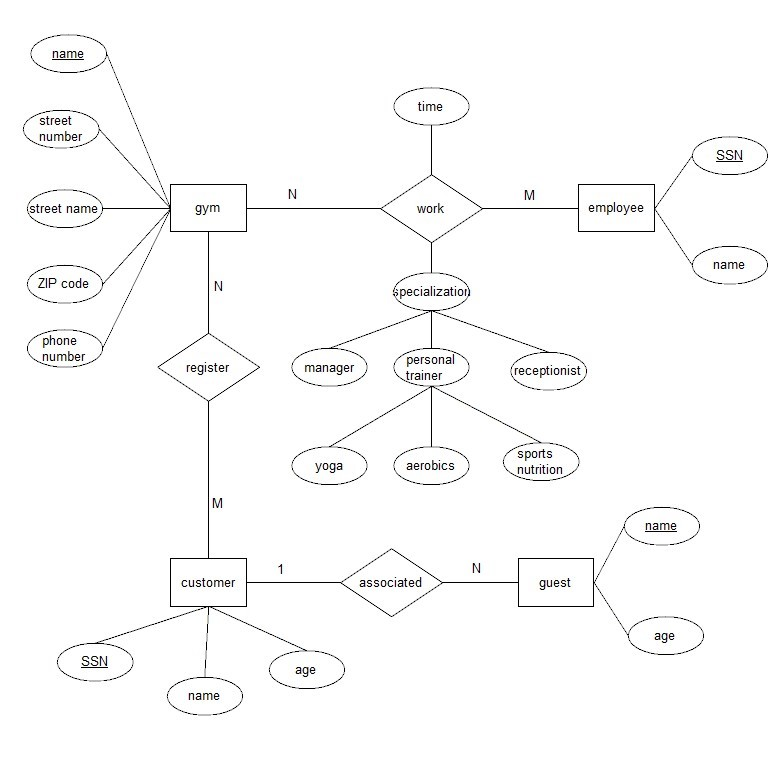
\includegraphics[scale=0.5]{1_1bk.jpg}
        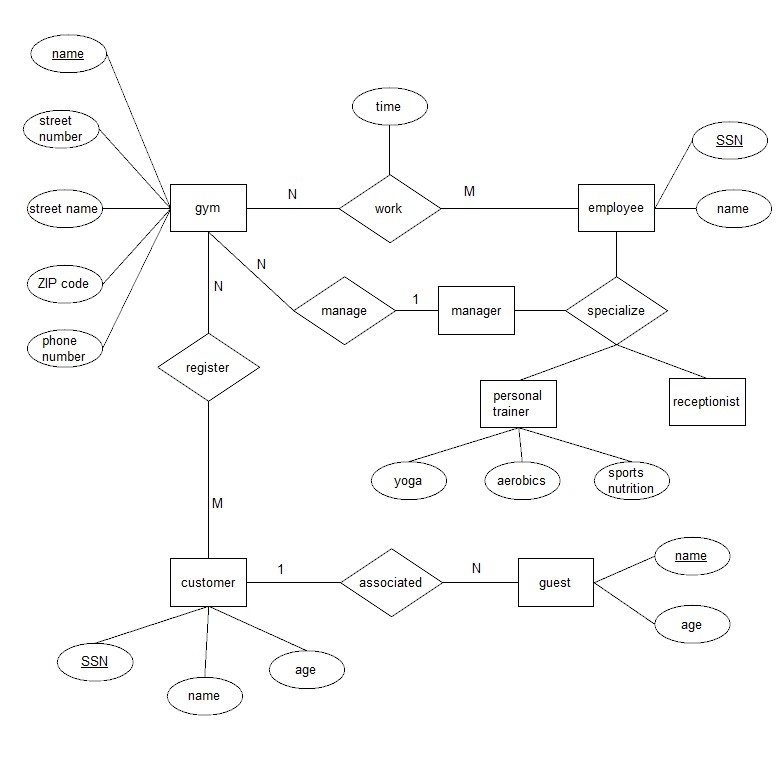
\includegraphics[scale=0.5]{1_2bk.jpg}
    \end{center}
    
    (2) Tables

    CREATE TABLE gyms(Gym\_name varchar(255) primary key, street\_number int, street\_name varchar(255), ZIP\_code int, phone\_number varchar(255))

    CREATE TABLE employees(Em\_SSN int primary key, Em\_name)

    CREATE TABLE work(Gym\_name varchar(255) foreign key, Em\_SSN varchar(255) foreign key, specialization varchar(255), certification\_type varchar(255))
    
    CREATE TABLE customer(C\_SSN int primary key, C\_name varchar(255), C\_age int)

    CREATE TABLE guest(Gu\_name varchar(255) primary key, Gu\_age)

    CRAETE TABLE register(Gym\_name varchar(255) foreign key, C\_SSN int foreign key)

    CREATE TABLE associated(C\_SSN int foreign key, Gu\_name varchar(255) foreign key)

    CREATE TABLE specialize(Em\_SSN int foreign kry, Specialization varchar(255) foreign key)

    CREATE TABLE manage(gym name varchar(255) foreign key, Em\_SSN int foreign key)

    CREATE TABLE personal\_trainer(Em\_SSN int primary\ key, certification\_type varchar(255))

    \subsection*{Problem 2}
    (1) SELECT sname FROM sup WHERE sid IN (

        SELECT sid FROM cat GROUP BY sid HAVING COUNT(*)=(
        
        SELECT DISTINCT COUNT(pid) FROM parts));\\
    (2) SELECT DISTINCT sid FROM cat,(

        SELECT pid,AVG(cost) as costt FROM cat GROUP BY cat.pid)catt

        WHERE cat.pid = catt.pid AND cat.cost $>$ catt.costt;\\
    (3) SELECT sname FROM sup WHERE sid IN(

        SELECT cat.sid FROM cat,(

        SELECT cat.sid,pid,MAX(cost) as maxc FROM cat GROUP BY cat.pid)maxcat

        WHERE cat.pid = maxcat.pid AND cat.cost = maxcat.maxc);\\
    (4) SELECT sid,pid FROM (

        SELECT sid,pid FROM cat GROUP BY sid HAVING COUNT(*)=1)pone 

        WHERE pone.pid=(SELECT pid FROM parts WHERE color='red');\\
    (5) SELECT sid FROM cat WHERE pid IN (

        SELECT pid FROM parts WHERE color='red' OR color='green');\\
    (6) SELECT cat1.pid,cat1.mcost FROM (

        SELECT cat2.pid,cat2.sid,MAX(cost) AS mcost FROM (

        SELECT cat.sid,cat.pid,cat.cost FROM cat WHERE EXISTS (

        SELECT sid FROM cat WHERE sid IN (

        SELECT t1.sid FROM (
        
        SELECT sid,pid,cost FROM cat WHERE pid=(
        
        SELECT pid FROM parts WHERE color='green'))t1

        INNER JOIN (SELECT sid,pid,cost FROM cat WHERE pid=(
            
        SELECT pid FROM parts WHERE color='red'))t2 
        
        ON t1.sid=t2.sid)))cat2 GROUP BY sid)cat1;


    \subsection*{Problem 3}
    (1) SELECT MovieName FROM Movies WHERE MovieID IN (

        SELECT MovieID IN MovieSupplier WHERE SupplierID IN (

        SELECT SupplierID FROM Suppliers WHERE SupplierName="Ben's Video" OR SupplierName="Video Clubhouse"))\\
    (2) SELECT MovieID FROM Inventory WHERE TapeID=(
        
        SELECT TapeID FROM Rentals WHERE Duration=MAX(Duration))\\
    (3) SELECT SupplierName FROM Suppliers WHERE SupplierID IN (
        
        SELECT SupplierID FROM MovieSupplier GROUP BY SupplierID HAVING COUNT(*)=(
            
        SELECT DISTINCT COUNT(*) FROM Movies))\\
    (4) SELECT MovieID FROM MovieSupplier WHERE EXISTS (
        
        SELECT MovieID FROM Inventory WHERE MovieSupplier.MovieID=Inventory.MovieID)\\
    (5) SELECT MovieName FROM Moivies WHERE MovieID IN (

        SELECT MovieID FROM Orders WHERE Copies>4)\\
    (6) SELECT CustomerID FROM Rentals WHERE TapeID=(
        
        SELECT TapeID FROM Inventory WHERE MovieID=(
            
        SELECT MovieID FROM Movies WHERE MovieName="Kung Fu Panda")
        
        OR MovieID=(SELECT MovieID FROM MovieSupplier WHERE SupplierID=(
            
        SELECT SupplierID FROM Suppliers WHERE SupplierName="Palm Video")))\\
    (7) SELECT MovieName FROM Moivies WHERE MovieID IN (
        
        SELECT MovieID FROM Orders WHERE Copies>1)\\
    (8) SELECT CustomerID FROM Rentals WHERE Duration>5\\

    (9) SELECT SupplierName FROM Suppliers WHERE SupplierID=(
        
        SELECT SupplierID FROM MovieSupplier WHERE price=MIN(price))\\
    (10) SELECT MovieName FROM Movies WHERE NOT EXISTS (
        
        SELECT MovieID FROM Inventory WHERE Movies.MovieID=Inventory.MovieID)
    
    \subsection*{Problem 4}
    a) The price in the new tuple which were 3 would be change to 1.5. And than the price of the product with purchaseID with 111 would be change to 1.5.\\
    b) The price in Purchase where purchaseID is 111 would be updated to 3 fisrt and then process the trigger. In this case, trigger basically dose nothing to the chart.\\
    c) INSTEAD OF shows exactly the same results with BEFORE. Actually, in MySQL, we use INSTEAD OF instead of BEFORE.




\end{document}